\input{symbol}
\documentclass[11pt]{article}
\usepackage{teschool14,epsfig}
\usepackage[utf8]{inputenc}
\usepackage[T1]{fontenc}
\usepackage{lmodern}
\usepackage{multirow}
\usepackage{amsmath}
\usepackage{amssymb}

\bibliographystyle{unsrt}
% for BibTeX - sorted numerical labels by order of
% first citation.

% A useful Journal macro
\def\Journal#1#2#3#4{{#1} {\bf #2}, #3 (#4)}

% Some useful journal names
\def\NCA{\em Nuovo Cimento}
\def\NIM{\em Nucl. Instrum. Methods}
\def\NIMA{{\em Nucl. Instrum. Methods} A}
\def\NPB{{\em Nucl. Phys.} B}
\def\PLB{{\em Phys. Lett.}  B}
\def\PRL{\em Phys. Rev. Lett.}
\def\PRD{{\em Phys. Rev.} D}
\def\ZPC{{\em Z. Phys.} C}

% Some other macros used in the sample text
\def\st{\scriptstyle}
\def\sst{\scriptscriptstyle}
\def\mco{\multicolumn}
\def\epp{\epsilon^{\prime}}
\def\vep{\varepsilon}
\def\ra{\rightarrow}
\def\ppg{\pi^+\pi^-\gamma}
\def\vp{{\bf p}}
\def\ko{K^0}
\def\kb{\bar{K^0}}
\def\al{\alpha}
\def\ab{\bar{\alpha}}
\def\be{\begin{equation}}
\def\ee{\end{equation}}
\def\bea{\begin{eqnarray}}
\def\eea{\end{eqnarray}}
\def\CPbar{\hbox{{\rm CP}\hskip-1.80em{/}}}
%temp replacement due to no font

%%%%%%%%%%%%%%%%%%%%%%%%%%%%%%%%%%%%%%%%%%%%%%%%%%
%                                                %
%    BEGINNING OF TEXT                           %
%                                                %
%%%%%%%%%%%%%%%%%%%%%%%%%%%%%%%%%%%%%%%%%%%%%%%%%%

\begin{document}
\vspace*{2cm}
\title{Study of Double Charm B Decays at LHCb}
\author{\Large\bf Renato Quagliani}

\address{Laboratoire de l'Accélérateur Linéaire (LAL), LHCb group,\\
 Orsay, France}

\begin{figure}
\begin{center}
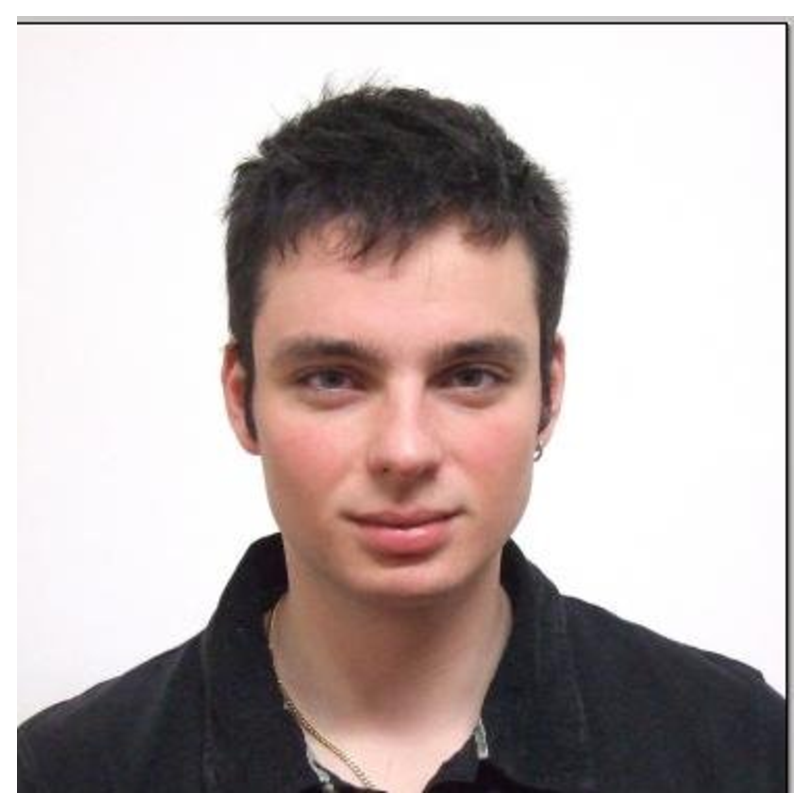
\includegraphics[bb=-306 1136 675 -1000, scale=0.265]{figs/07b901e.eps}
\end{center}
\end{figure}


\maketitle\abstracts{
The work presented consists in a preliminary study for the measurement of the branching ratio of the doubly charmed decay ${ B }^{ 0 }\rightarrow { D }^{ 0 }\overline { { D }^{ 0 } } { K }^{ *0 } + C.C.$ (never measured and observed so far) using the ${ B }^{ + }\rightarrow { D }^{ 0 }\overline { { D }^{ 0 } } { K }^{ + } +C.C.$ as reference channel. The $D$ mesons are reconstructed through $\Dzch +c.c$.
 The $LHCb$ experiment 2011 and 2012 data have been used for a total integrated luminosity of 3 $fb^{-1}$ .
A preliminary study on the reference channel $B^{+}\rightarrow D^{0}\overline{D^{0}}K^{+}$ has been performed, together with a partial \textit{Dalitz} analysis. The $B$ mesons double charm decays have been introduced to explain the discrepancy between semileptonic branching ratio of $B$ decays and the observed number of charmed mesons in $B$ decays. Nowadays, there are some of the decay modes which has not been observed and the $\Bzch$ is one of them.
More interest about this topology of decay concern the search of exotic structures above the open charm thresholds ($>2M_{D}$). In this mass region observed states and charmonium ($c\overline{c}$ bound states) predicted one are in disagreement and channels as the one considered here can lead interesting results in this domain.
%For the reference channel ${ B }^{ + }\rightarrow { D }^{ 0 }\overline { { D }^{ 0 } } { K }^{ + } +C.C.$ the data sample has been studied and subjected to two different selection stages: 
%\begin{itemize}
%\item Pre-selection of  ${ B }^{ + }\rightarrow { D }^{ 0 }\overline { { D }^{ 0 } } { K }^{ + } +C.C.$ where the $D$ mesons are reconstructed through the decay modes $D^{0}\rightarrow K^{-} \pi^{+}$ and $\overline{D}^{0} \rightarrow K^+ \pi^-$.
%\item Selection and sample purification of  ${ B }^{ + }\rightarrow{ D }^{ 0 }\overline{ { D }^{ 0 } }{ K }^{ + } +C.C.$  with the help of $MultiVariate$ $Analysis$ (MVA) techniques.
%\end{itemize}
%After these two steps, a preliminary $Dalitz$ study has been performed in the purified sample for the  ${ B }^{ + }\rightarrow { D }^{ 0 }\overline { { D }^{ 0 } } { K }^{ + } +C.C.$ channel.
%For the  ${ B }^{ 0 }\rightarrow { D }^{ 0 }\overline { { D }^{ 0 } } { K }^{ *0 }$ channel only the Pre-Selection step has been done because $MultiVariate$ $Analysis$ techniques can only be performed using a signal-like sample. The MC sample has been requested to the \textit{LHCb} collaboration and it becomes available only in October 2014.
%In addition, other double charm decays characterized by the $b\rightarrow c \overline{c}s$ transition have been found and they have been added to the MC repository of the \textit{LHCb} software. These decay modes which will be listed in the perspective section of the chapter 4 can be used in future for exotic mesons search, isospin relation tests and also for background studies.
}

\section{${ B }\rightarrow { D }^{ (*)} { D }^{ (*) } { K }^{ (*) }$ Decays : topology and possible physics studies}

At the quark level, the  $B^{+}\rightarrow D^{0} \overline{D}^{0} K^{+} +c.c.$ 
$B^{0}\rightarrow D^{0} \overline{D}^{0} K^{\ast 0}  +  c.c.$ are generally described by the \textit{CKM} favoured weak transition $\overline{b} \rightarrow \overline{c} W^{+} \rightarrow \overline{c} c \overline{s}$ with additional $u\overline{u}$(or $d\overline{d} $ ) quarks coming from the \textit{QCD} vacuum.\footnote{These decay modes have been introduced due to the so called \textit{Charm counting puzzle}, i.e., theoretical discrepancy between the semileptonic branching ratio of $B$ decays with the number of charmed hadrons produced in $B$  decays.}  The relevant Feynman diagrams for such decay modes are shown in Fig \ref{quarks}.
\begin{figure}[h!]
\begin{center}
\includegraphics[ width=0.5\textwidth]{figs/Feynman2.png}
\caption{Leading order Feynman diagrams for $\Bpch$. On the right the colour-favoured mode ($u\overline{u}$ from \textit{QCD} vacuum can have 3 different colour assignment), on the left the colour suppressed mode (once the spectator quark colour is fixed, all the other are fixed). For $\Bpch$ both the modes can occur while for the $\Bzch$ only the suppressed mode can occurs.}\label{quarks}
\end{center}
\end{figure}


Hadrons are colourless objects so the decay modes containing $D^{(\ast)}$ as the ones of interest are produced in majority through Internal (colour suppressed) and/or external modes (colour favoured). The reference channel occur through both of them while the $\Bzch$ only internally.

The major study, which can be done through these decay modes, is the spectroscopy of $c\overline{s} $ and $c\overline{c}$ states. Resonances coming from  $D^{\ast}_{s} \rightarrow D^{(\ast)} K^{(\ast)}$ and  $X \rightarrow D^{(\ast)}D^{(\ast)}$ can be studied in 3-body decays through \textit{Dalitz Amplitude Analysis technique}. The physics case is more interesting for the second category.\footnote{ There are several discrepancies between observed states and predicted one in the $X \rightarrow D^{(\ast)}D^{(\ast)}$ and the nature of some of the observed one is not clear and unambiguously defined yet.}.
The weak decay of interest is isospin conserving, so through isospin decomposition of amplitudes one can test the factorization theorem for three body decays and predict the branching ratio of other similar channels just measuring one of them.

\section{Analysis performed}
The goal of the analysis is to measure the $\mathcal{B.R.}$ of the  $\Bzch$. The way to perform this measurement is to refer the value to a reference channel. The master formula that one has to use to perform this measurement is \footnote{Several factors disappear}:

\tiny \begin{equation}\label{1}
\begin{split} 
\frac { { N }_{ event }\left( B^0\rightarrow \overline{D}^0 D^0 K^{\ast 0} \right)  }{ { N }_{ event }\left( B^+\rightarrow \overline{D}^0 D^0 K^{+} \right)  }&  = \frac{\mathcal{L}}{\mathcal{L}}\times \frac{\sigma_{b\overline{b}}}{\sigma_{b\overline{b}}}   \frac { 2 \times { f }_{ { B }^{ 0 } } }{ 2 \times { f }_{ { B }^{ + } } } \times \frac { \mathcal{B.R.}\left( B^0\rightarrow \overline{D}^0 D^0 K^{\ast 0} \right)  }{ \mathcal{B.R.}\left(B^+\rightarrow \overline{D}^0 D^0 K^{+} \right)  } \times \frac { \mathcal{B.R.}\left( \Dzch \right)  }{ \mathcal{B.R.}\left( \Dzch \right)  }  \\   & \times \frac { \mathcal{B.R.}\left( \Dzbarch \right)  }{ \mathcal{B.R.}\left( \Dzbarch \right)  } \times \frac { \mathcal{B.R.}\left( \Kstch \right)  }{ 1 } \times \frac { { \varepsilon ^{\ast} }_{ tot } }{ {  \varepsilon^{\ast \ast} }_{ tot } }
\end{split} 
\end{equation}
\normalsize where
\tiny \begin{equation} \label{epsilon}
 \varepsilon_{ tot } = \varepsilon_{geometric}\times \varepsilon_{trigger}\times \varepsilon_{Selection}
\end{equation}
\normalsize After a pre-selection\footnote{Based on the truth matched candidates in the Monte Carlo simulation} and using multivariate analysis (\textit{MVA} )technique\footnote{It relies in machine learning algorithms able to disentangle and classify a signal-like and background like sample knowing the values of a set of input variables.} it has been possible to obtain a rather clean sample of $B^{+}$ mesons in the $\Bpch$ as shown in fig \ref{Bmass}.
\begin{figure}[h!]
\begin{center}
\includegraphics[ width=0.5\textwidth]{figs/BDTCatMassB.pdf}
\caption{Reconstructed $B$ mass spectrum for  the 2011 and 2012 LHCb data in the $B^{\pm} \rightarrow D^{0} \overline{D}^{0} K^{\pm}$ channel. \it{Data Stripping + Filter} are the pre-selected \textit{B} candidates. The \it{BDTCat} is the \it{MVA} classifier which permits to separate background-like and signal-like candidates. The cut value \it{-0.15} has been chosen maximising the $\frac{S}{\sqrt{S+B}}$ figure of merit. (here $\sim 40$). The two peaks below the nominal $B^{+}$ mass  consists into reconstructed $D$ mesons from the strong $D^{\ast}\rightarrow D \pi$ decay where the $\pi$ is outside the LHCb acceptance.}\label{Bmass}
\end{center}
\end{figure}

Using the sample of $B$ candidates obtained,  a preliminary Dalitz analysis has been done looking to the \textit{2-D} plot build using the $M^{2}_{A+B}$ and $M^{2}_{B+C}$ invariant masses distributions out of a 3-body decay $X\rightarrow ABC$ decay. The obtained plot is shown in Fig \ref{Dalitz}.
\begin{figure}[h!]
\begin{center}
\includegraphics[ width=0.7\textwidth]{figs/Dalitz1.pdf}
\caption{$\Bpch$ Dalitz Plot of $(D^{0}\overline{D}^{0})$ vs. $(D^{0}K^{+}+c.c.)$. The accumulation of events on the top-left part are related to $B^{+}\rightarrow \psi(3770)K^{+}\rightarrow D^{0}\overline{D}^{0} K^{+}$ in fact the $\psi(3770)$ has a $J=1$ and the corresponding typical pattern is the one that can be seen (two peaks). In addition another resonance is present in the central horizontal line and it correspond to a $J=1$ resonance due to $D^{*}_{s1}(2700)\rightarrow D^{0}K^{\pm}$.}\label{Dalitz}
\end{center}
\end{figure}

\section{Result}
The analysis is still on going and only a full amplitude analysis will tell if there are other structures in the $\Bpch$ and in the $\Bzch$. The first goal will be the measurement and the observation of the $\Bzch$. The presented work already highlights the presence of resonant structure in the $D^{0} \rightarrow \overline{D} ^{0} $ spectrum compatible with the $\psi (3770)$ (should be also present in $\Bzch$) and also a peak structure in the $D^{0} K^{+} $ invariant mass spectrum compatible with the $D^{*}(2700)^{+}$ (this should not appear in $\Bzch$ ).

In addition , a very preliminary mass spectrum of the $B^{0}$ has been obtained (not shown here) with a roughly estimated yield of 300 events compatible with a predicted yield of $\sim 100 $ events.

\section{Bibliography}
Further details about this work and a complete description of the physics case can be found here:
\begin{itemize}
\item \textit{Renato Quagliani, Master Degree thesis, https://dbms.ilrt.bris.ac.uk/media/user/334129/tesi.pdf}
\end{itemize}

\end{document}


 




%%%%%%%%%%%%%%%%%%%%%%
% End of teschool13.tex  %
%%%%%%%%%%%%%%%%%%%%%%

